% feasibility-report.tex: 可行性报告
% Copyright (C) 2022 吴骏东, 张子辰, 蓝俊玮, 郭耸霄 and 陈建绿
% All rights reserved.

% This file is part of Runikraft. Runikraft is free software,
% which is released under the BSD 3-Clause License, see LICENSE for detail.
% Runikraft is provided ``as is'', without any express or implied warrenties.

% The reports of Runikraft are released under the Creative Commons
% Attribution 4.0 International License; see report/LICENSE for detail.
\documentclass[UTF8,fontset=none,linespread=1.15]{ctexart}
\ctexset
{
    section/format={\Large\sffamily\bfseries},
    subsection/format+={\sffamily},
    subsubsection/format+={\itshape}
}
\setCJKmainfont[ItalicFont={KaiTi},BoldItalicFont={KaiTi},
BoldItalicFeatures={FakeBold=3}]{Noto Serif CJK SC}
\setCJKsansfont[BoldFont={Noto Sans CJK SC Bold},
BoldItalicFont={Noto Sans CJK SC Bold},
AutoFakeSlant]{Noto Sans CJK SC DemiLight}
\setCJKmonofont[AutoFakeBold=3,AutoFakeSlant]{FangSong}
\setmainfont{cmun}[Extension=.otf,UprightFont=*rm,
ItalicFont=*ti,BoldFont=*bx,BoldItalicFont=*bi]
\setsansfont{cmun}[Extension=.otf,UprightFont=*ss,
ItalicFont=*si,BoldFont=*sx,BoldItalicFont=*so]
\setmonofont{cmun}[Extension=.otf,UprightFont=*btl,
ItalicFont=*bto,BoldFont=*tb,BoldItalicFont=*tx]
%Computer Modern Unicode 的\textasciitilde和\~{}的高度相同,所以用\tildechar表示居中的波浪线~
\newcommand{\tildechar}{\raisebox{-0.35em}{\textasciitilde}}
\usepackage[a4paper,hmargin=1.2in,vmargin=1in]{geometry}
\usepackage{graphicx,tikz,float,subfig,multicol,makecell,multirow,longtable}
\usepackage[normalem]{ulem}
\usepackage{CJKfntef}
\usepackage[perpage]{footmisc}

%目录, 参考了OSH-2021/x-sBPF
\usepackage{titletoc}
\titlecontents{section}[2em]{\addvspace{1.3mm}\bfseries}{%
\contentslabel{2.0em}}{}{\titlerule*[5pt]{$\cdot$}\contentspage}
\titlecontents{subsection}[4.2em]{}{\contentslabel{2.5em}}{}{%
\titlerule*[5pt]{$\cdot$}\contentspage}
\titlecontents{subsubsection}[7.2em]{}{\contentslabel{3.3em}}{}{%
\titlerule*[5pt]{$\cdot$}\contentspage}

%代码环境
\usepackage{listings}
\lstset{basicstyle={\normalfont\ttfamily},breaklines,tabsize=4}

\usepackage{enumitem}
\setlistdepth{5}
\renewlist{enumerate}{enumerate}{5}
\setlist{itemsep=0pt,partopsep=0pt,parsep=0pt,topsep=0pt}
\setlist[enumerate,1]{label=\arabic*.}
\setlist[enumerate,2]{label=(\arabic*)}
\setlist[enumerate,3]{label=\textcircled{\arabic*}}
\setlist[enumerate,4]{label=(\textit{\roman*})}
\setlist[enumerate,5]{label=\textit{\alph*})}

\usepackage[colorlinks,unicode,pdfstartview={FitH}]{hyperref}
\hypersetup
{
  pdftitle={2022春 操作系统原理与设计(H) x-runikraft小组 可行性报告},
  pdfauthor={吴骏东; 张子辰; 蓝俊玮; 郭耸霄; 陈建绿}
}

%带圈数字,它必须在hyperref之后载入
\usepackage{xunicode-addon}
\makeatletter
\xeCJKDeclareCharClass{CJK}{"24EA, "2460->"2473, "3251->"32BF,"24B6->"24E9,"2160->"217F}
\newfontfamily\EnclosedNumbers{Noto Serif CJK SC}
\AtBeginUTFCommand[\textcircled]{\begingroup\EnclosedNumbers}
\AtEndUTFCommand[\textcircled]{\endgroup}
\makeatother

\makeatletter
\let\textcircled@old\textcircled
\protected\def\textcircled#1{%
	\expandafter\textcircled@old\expandafter{\expanded{#1}}}
\makeatother
\makeatletter
\renewcommand\@makefntext[1]{%
	\setlength\parindent{0.75\ccwd}\selectfont
	\@thefnmark\ #1}
\makeatother
\renewcommand*\thefootnote{\textcircled{\arabic{footnote}}}
\renewcommand{\lstlistingname}{代码}

%上标+引用
\let\nosupcite\cite
\renewcommand*{\cite}[1]{\textsuperscript{\nosupcite{#1}}}

%章节作者
\newcommand{\sectionauthor}[1]{%
\vspace*{-5ex}
\noindent\textrm{\hfill\textit{by #1}}
\vspace*{2ex}\par}
%\renewcommand{\today}{2022年4月5日}

\begin{document}
\sffamily %为方便屏幕阅读,文档主要使用无衬线字体
\title{\bfseries Runikraft小组\quad 可行性报告}
\author{吴骏东\and 张子辰\and 蓝俊玮\and 郭耸霄\and 陈建绿}
\date{\today}
\maketitle

\tableofcontents

\section{理论依据}
\section{技术依据}
\section{创新点}
\section{概要设计}
Runikraft的架构与Unikraft几乎相同。
\begin{figure}[!hbt]
\centering
\begin{minipage}{0.49\linewidth}
\centering
\includegraphics[width=\linewidth]{assets/Unikraft-architecture.png}
\caption{Unikraft的架构}\label{fig:unikraft-arch}
\end{minipage}
\begin{minipage}{0.49\linewidth}
\centering
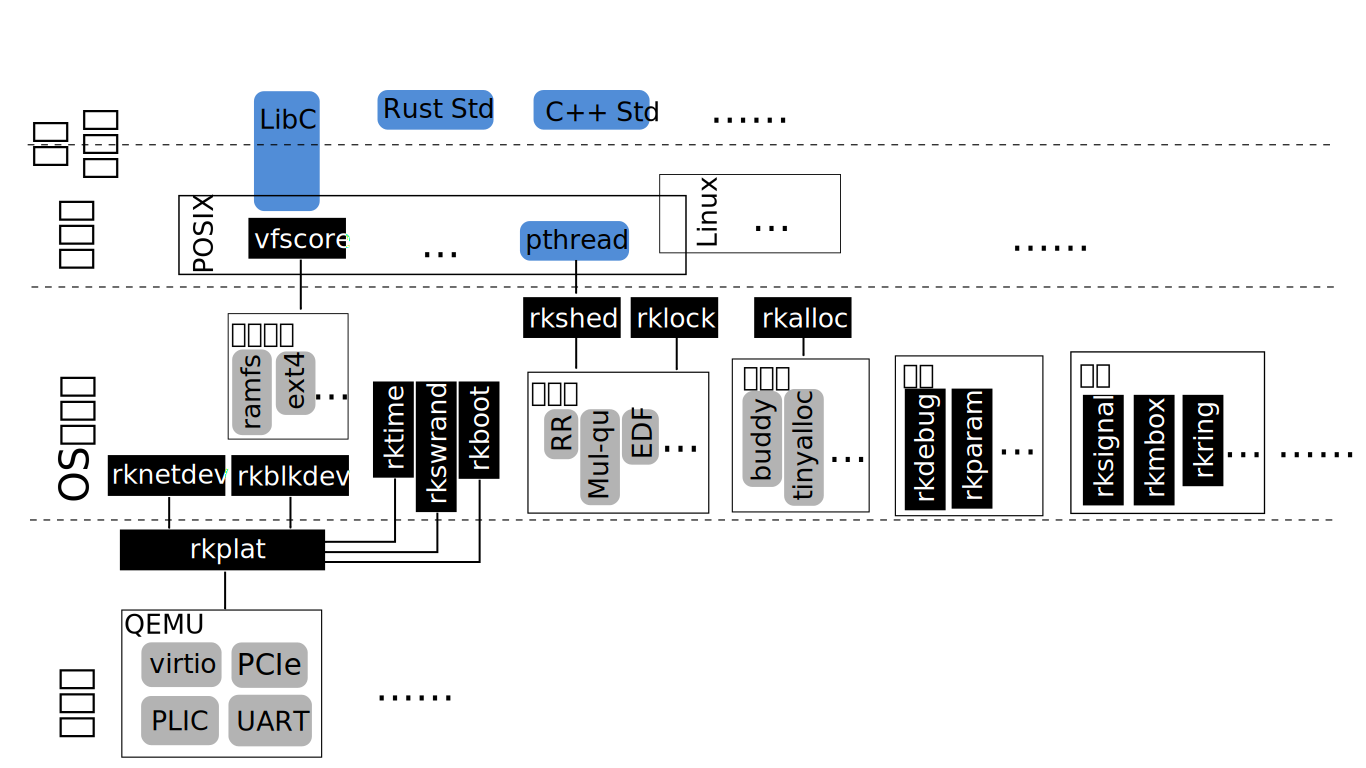
\includegraphics[width=\linewidth]{assets/Runikraft-architecture.pdf}
\caption{Runikraft的架构}\label{fig:runikraft-arch}
\end{minipage}
\end{figure}
平台层将不同的平台封装成通用的\texttt{rkplat} API,它提供与平台/架构密切相关的功能,
比如外设驱动、外中断处理、内存分页、定时器、原子操作、内存屏障,我们只计划支持RISC-V+QEMU virt
一种平台。如果时间不足,我们可以将现成的OpenSBI\cite{bib:sbi}\cite{bib:opensbi}封装成\texttt{rkplat} API。

\texttt{rknetdev}、\texttt{rkblkdev}、\texttt{rktime}、\texttt{rkswrand}、\texttt{rkboot}
五个APIs的功能与平台密切相关,
但是为了降低开发和维护难度,它们并没有直接实现,而是在\texttt{rkplat}提供的初级抽象的基础上实现。
\texttt{rknetdev}和\texttt{rbblkdev}对应图\ \ref{fig:unikraft-arch}\ 的⑦和⑧,
它们分别提供网络设备和块设备的支持。
%与Unikraft的实现类似,这两个APIs的构造函数的参数接受指向\texttt{trait RKplat}的指针。
\texttt{rktime}提供获取和修改系统时间的API,\texttt{rkswrand}提供密码学安全的随机数,
\texttt{rkboot}负责完成系统的初始化并将控制权转交给用户的代码。

\texttt{rkshed}和\texttt{rklock}是两个与调度器有关的APIs,前者负责创建、调度、撤销线程,后者负责线程间
的同步和互斥。Runikraft支持多种调取器,比如,图\ \ref{fig:runikraft-arch}\ 中的RR的时间片轮转调度器、
Mul-qu是多重队列调取器、EDF是截止日期有限调度器。我们计划先实现RR调度器。当然,为了系统镜像的轻量性,
用户可以不使用任何调取器,这时,\texttt{rkshed}和\texttt{rklock}会被编译成空API,创建线程的行为
将和函数调用相同。这保证了大部分使用仅仅并行加速的程序仍然能正确运行。

Runikraft选择性地提供线程通信模块,如UNIX风格的信号(\texttt{rksignal}),信箱(\texttt{rkmbox}),
无锁的环形缓冲队列(\texttt{rkring})。

我们目前没有计划区分线程和进程,Runikraft的线程同时具有传统的OSes的线程和进程的特性:
线程之间没有隔离措施,但是线程之间又可以使用进程通信的方法更安全地同步。

\texttt{rkalloc}是分配器API,它的后端可以是\texttt{buddy}、\texttt{tinyalloc}、\texttt{tlsf}、
\texttt{mimalloc}等分配器。
不过,我们可能只会实现其中的一个。

Runikraft还提供了一些工具模块,比如调试工具\texttt{rkdebug}、命令行参数分析工具\texttt{rkparam}。

文件系统支持虽然是OS元件的一部分,但是考虑到文件系统之前的功能不尽相同,完全隐藏差异会影响用户的操作能力,
所以OS元件层并没有提供统一的文件系统API。

\section*{许可协议}
本文档以知识共享署名 4.0 国际 (CC BY 4.0)许可证发布。

\vspace{2ex}
\noindent\textbf{\large 您可以自由地}:
\begin{description}
\item[共享] 在任何媒介以任何形式复制、发行本作品;
\item[演绎] 修改、转换或以本作品为基础进行创作
在任何用途下,甚至商业目的。
\end{description}

\vspace{2ex}
\noindent\textbf{\large 惟须遵守下列条件}:
\begin{description}
\item[署名] 您必须给出适当的署名,提供指向本许可协议的链接,
同时标明是否(对原始作品)作了修改。您可以用任何合理的方式来署名,
但是不得以任何方式暗示许可人为您或您的使用背书。
\item[没有附加限制] 您不得使用法律术语或者技术措施,从而限制其他人
做许可协议允许的事情。
\end{description}

\vspace{2ex}
\noindent\textbf{\large 声明}:

您不必因为公共领域的作品要素而遵守许可协议,或者您的使用被可适用的例外或限制所允许。

不提供担保。许可协议可能不会给与您意图使用的所必须的所有许可。
例如,其他权利比如形象权、隐私权或人格权可能限制您如何使用作品。

本许可证的全文位于:\\
\centerline{\url{https://creativecommons.org/licenses/by/4.0/legalcode.zh-Hans}}

\begin{thebibliography}{99}
\bibitem{bib:sbi} \url{https://github.com/riscv-non-isa/riscv-sbi-doc/releases/tag/v1.0.0}
\bibitem{bib:opensbi} \url{https://github.com/riscv-software-src/opensbi/releases/tag/v1.0}
\end{thebibliography}
\end{document}